\chapter{Results}\label{cha:results}

This chapter presents the results from the experiments conducted to evaluate the performance of the unsupervised learning methods investigated in this thesis. 

\section{Depth and ego motion}

\begin{figure}[H]
	\centering
	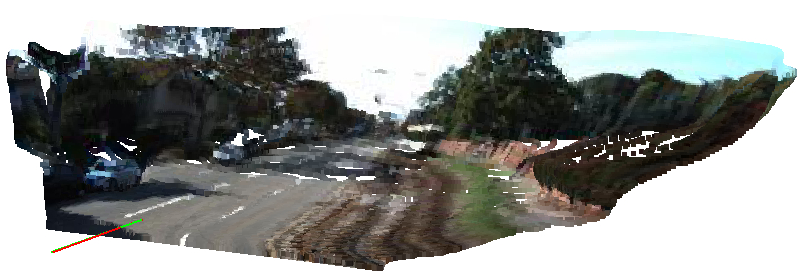
\includegraphics[width=1.0\textwidth]{3drender}
	\caption{3D render of colorized depth map}
	\label{fig:3drender}
\end{figure}

\begin{figure}[H]
	\centering
	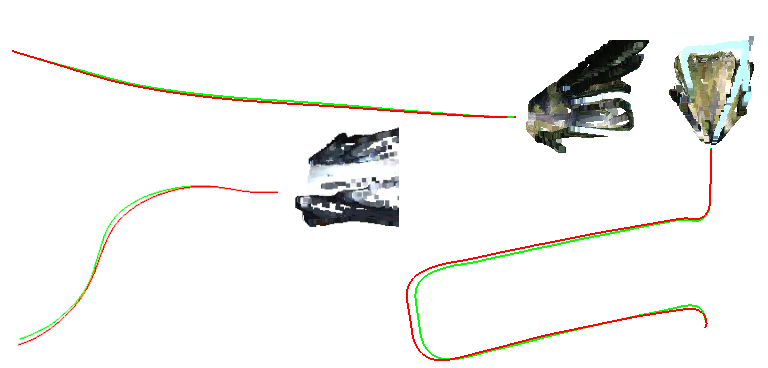
\includegraphics[width=0.8\textwidth]{motion2}
	\caption{3D visualization of the camera movement in three different image sequences. The green lines are the ground truth and the red lines are the predicted camera trajectories.}
	\label{fig:movement}
\end{figure}


\begin{table}[H]
\centering
\begin{tabular}{|l|c|c||c|c||c|c||c|c|c|c|}
\hline
C & Net & DS & Edge & Norm & Expl & Stat & SSIM & Comb & US \\
\hline
1 & SL & K &  &  &  &  &  & avg &  \\
\hline
2 & SL & K &  &  & $ \times $ &  &  & avg &  \\
\hline
3 & SL & K &  &  &  & $ \times $ &  & avg &  \\
\hline
4 & SL & K & $ \times $ &  &  & $ \times $ &  & avg &  \\
\hline
5 & SL & K & $ \times $ &  &  & $ \times $ & $ \times $ & min &  \\
\hline
6 & SL & K & $ \times $ & $ \times $ &  & $ \times $ & $ \times $ & min &  \\
\hline
7 & SL & K & $ \times $ & $ \times $ &  & $ \times $ & $ \times $ & min & $ \times $ \\
\hline
8 & SL & L & $ \times $ & $ \times $ &  & $ \times $ & $ \times $ & min & $ \times $ \\
\hline
9 & M2 & K &  &  &  & $ \times $ &  & avg &  \\
\hline
10 & M2 & K & $ \times $ & $ \times $ &  & $ \times $ & $ \times $ & min &  \\
\hline
11 & M2 & K & $ \times $ & $ \times $ &  & $ \times $ & $ \times $ & min & $ \times $ \\
\hline
12 & M2 & L & $ \times $ & $ \times $ &  & $ \times $ & $ \times $ & min & $ \times $ \\
\hline
\end{tabular}
\caption{All configurations of the depth and ego motion network that were evaluated. The C column identifies the specific configuration. The Net column shows which architecture was used, either SL for SfmLearner or M2 for Monodepth2. The DS column shows which dataset was used during training, either K for Kitti or L for Lyft. The Edge column indicates if the edge aware smoothing loss term $\mathcal{L}_{edge}$ was used. The Norm column indicates if depth map normalization was used. The Expl column indicates if an explainability mask was used. The Stat column indicates if a mask to remove stationary pixels from the loss was used. The SSIM column indicates if $\mathcal{L}_{ps}$ was used, otherwise just $\mathcal{L}_{p}$. The Comb column shows which methods was used to combine the loss terms from the two source images, either the average or the minimum loss across frames. The US column indicates that up scaling of the depth maps in the pyramid was used, otherwise the target frame was down scaled to match the size of the smaller depth maps in the pyramid.}
\label{table:configurations}
\end{table}


\begin{table}[H]
\centering
{\setlength{\tabcolsep}{0.4em}
\begin{tabular}{|r|r|c||l|l|l|l||l|l|l||l|}
\hline
E & C & DS & AbsRel & SqRel & RMSE & RMSLE & $1.25$ & $1.25^2$ & $1.25^3$ & Ego \\
\hline
1 & 1 & K & 0.174 & 1.405 & 4.829 & 0.249 & 0.784 & 0.920 & 0.964 & 0.024 \\
\hline
2 & 2 & K & 0.179 & 1.686 & 4.880 & 0.252 & 0.782 & 0.919 & 0.961 & 0.021 \\
\hline
3 & 3 & K & 0.140 & 0.793 & 4.549 & 0.217 & 0.818 & 0.939 & 0.976 & 0.020 \\
\hline
4 & 4 & K & 0.143 & 0.819 & 4.708 & 0.222 & 0.810 & 0.937 & 0.975 & 0.022 \\
\hline
5 & 5 & K & 0.133 & 0.727 & 4.305 & 0.204 & 0.843 & 0.950 & 0.979 & 0.023 \\
\hline
6 & 6 & K & 0.137 & 0.797 & 4.282 & 0.208 & 0.837 & 0.948 & 0.977 & 0.024 \\
\hline
\hline
7 & 7 & K & 0.135 & 0.778 & 4.248 & 0.208 & 0.841 & 0.948 & 0.997 & 0.020 \\
\hline
8 & 7 & L & 0.340 & 7.811 & 23.071 & 0.447 & 0.457 & 0.734 & 0.868 & 0.043 \\
\hline
9 & 8 & K & 0.512 & 5.185 & 10.757 & 0.611 & 0.305 & 0.549 & 0.732 & 0.495 \\
\hline
10 & 8 & L & 0.739 & 20.236 & 31.859 & 0.773 & 0.240 & 0.434 & 0.587 & 1.324 \\
\hline
\hline
11 & 9 & K & \textbf{0.125} & \textbf{0.697} & 4.298 & 0.203 & 0.845 & 0.948 & 0.979 & 0.021 \\
\hline
12 & 10 & K & 0.126 & 0.714 & 4.018 & \textbf{0.194} & \textbf{0.860} & \textbf{0.958} & \textbf{0.982} & \textbf{0.019} \\
\hline
\hline
13 & 11 & K & 0.132 & 0.769 & \textbf{3.966} & 0.196 & 0.859 & 0.957 & 0.981 & \textbf{0.019} \\
\hline
14 & 11 & L & 0.304 & 7.019 & 21.907 & 0.414 & 0.518 & 0.775 & 0.886 & 0.042 \\
\hline
\hline
15 & 12 & K & 0.322 & 3.177 & 7.179 & 0.378 & 0.549 & 0.797 & 0.906 & 0.036 \\
\hline
16 & 12 & L & 0.303 & 8.051 & 19.312 & 0.385 & 0.637 & 0.827 & 0.906 & 0.059 \\
\hline
\end{tabular}}
\caption{All the experiments measuring the performance of the different configurations in Table \ref{table:configurations}. The E column identifies a specific experiment. The C column shows which configuration was used. The DS column shows which Dataset was used during testing, K for Kitti and L for Lyft. The dataset used during testing differs from the one used during training in some experiments. The AbsRel, SqRel, RMSE and RMSLE columns are the depth error metrics described in section \ref{sec:depthmetrics}, smaller is better. The $1.25$, $1.25^2$ and $1.25^3$ columns are the depth accuracy metrics described in section \ref{sec:depthmetrics}, larger is better. The Ego column is the camera ego motion error metric described in section \ref{sec:egometric}.}
\label{table:experiments}
\end{table}

TODO: Describe the improvements (if any) seen by applying each additional method for depth prediction and explain why this could be....

\iffalse
\begin{figure}[H]
	\centering
	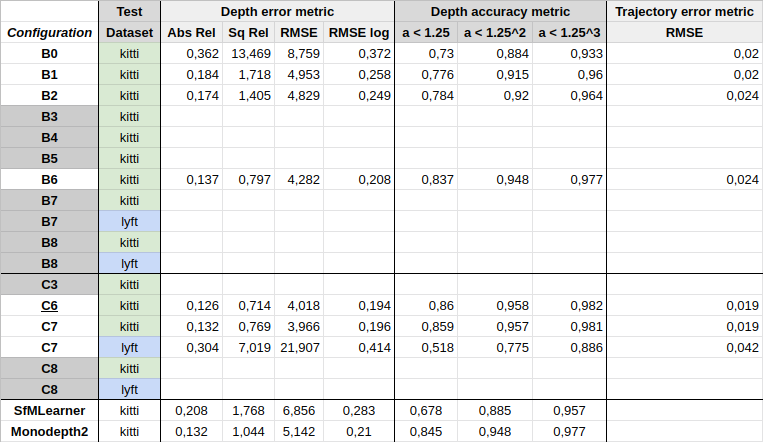
\includegraphics[width=1.0\textwidth]{evaluation}
	\caption{Evaluation metrics when testing the configurations on the testing split of the datasets}
	\label{fig:evaluation}
\end{figure}
\fi

\clearpage

\begin{figure}[H]
	\centering
	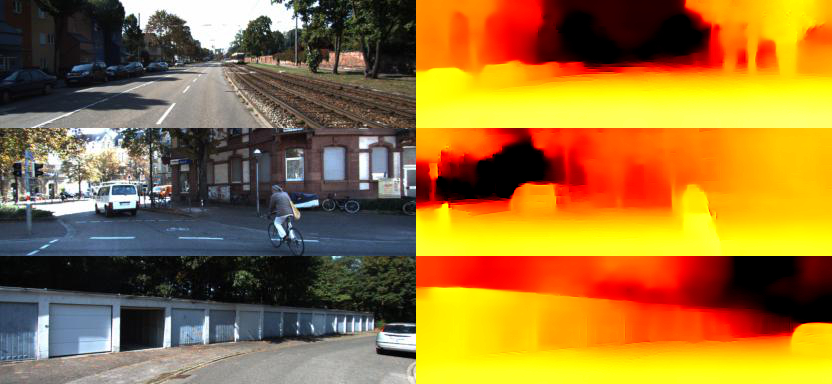
\includegraphics[width=1.0\textwidth]{depthmaps}
	\caption{Examples from the Kitti dataset}
	\label{fig:depthmapskitty}
\end{figure}

\begin{figure}[H]
	\centering
	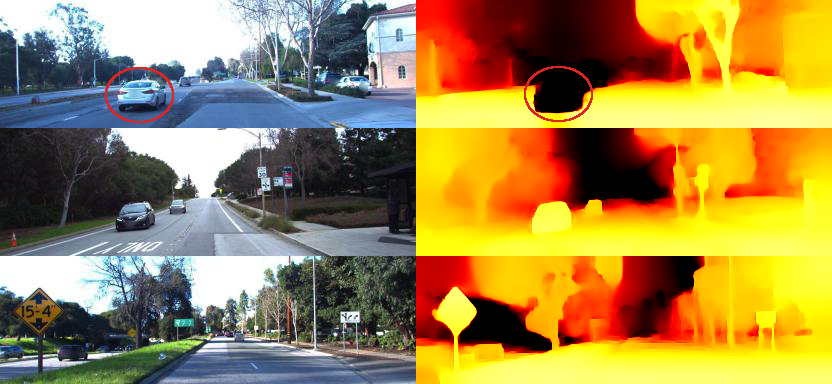
\includegraphics[width=1.0\textwidth]{depthmapslyft}
	\caption{Examples from the Lyft dataset}
	\label{fig:depthmaplyft}
\end{figure}

\begin{figure}[H]
	\centering
	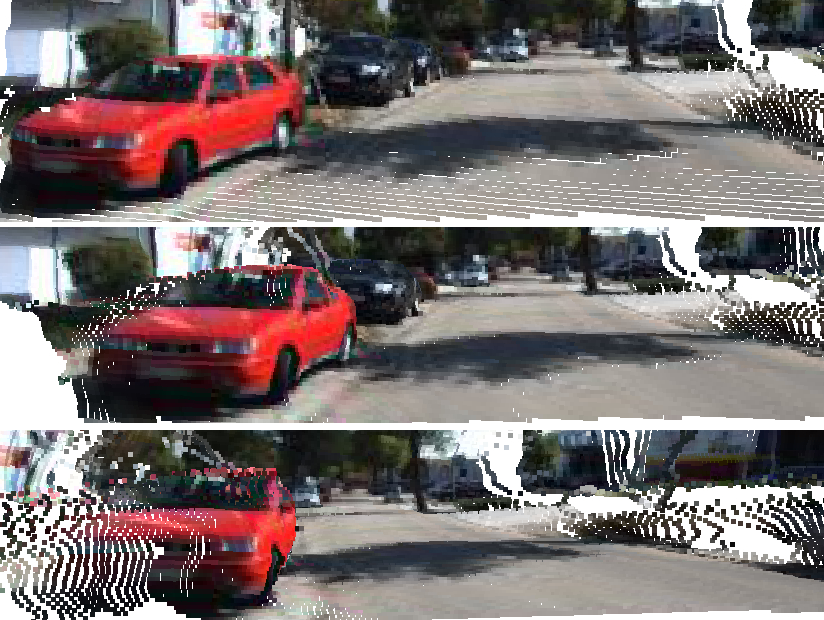
\includegraphics[width=0.8\textwidth]{3dseq}
	\caption{3D visualization from 3 different angles of the same frame in the kitti dataset.}
	\label{fig:3dseq}
\end{figure}

\section{Keypoint detection}

\begin{figure}[H]
	\centering
	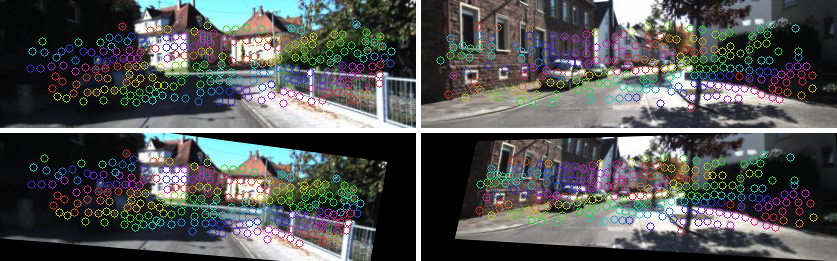
\includegraphics[width=1.0\textwidth]{point1}
	\caption{Results from the keypoint prediction network. The top row are the original input images fed to branch A, and bellow are the transformed images fed to branch B. Circles that are the same color have matching descriptors.}
	\label{fig:point1}
\end{figure}

\begin{table}[H]
\centering
\begin{tabular}{|l|l|l|l|l|l|l|}
\hline
Method & RS $\uparrow$ & LE $\downarrow$ & MS $\uparrow$ & CMR $\uparrow$ & Nt & Nm \\
\hline
UnsuperPoint & 0.796 & \textbf{0.666} & \textbf{0.488} & \textbf{0.834} & 338 & 203 \\
ORB & \textbf{0.841} & 0.764 & 0.302 & 0.564 & 310 & 171 \\
\hline
\end{tabular}
\caption{Experiments measuring the performance of keypoint detection methods.}
\label{table:pointsbenchmark}
\end{table}

TODO: Describe what the results are showing....

\section{Consensus maximization}

\begin{figure}[H]
	\centering
	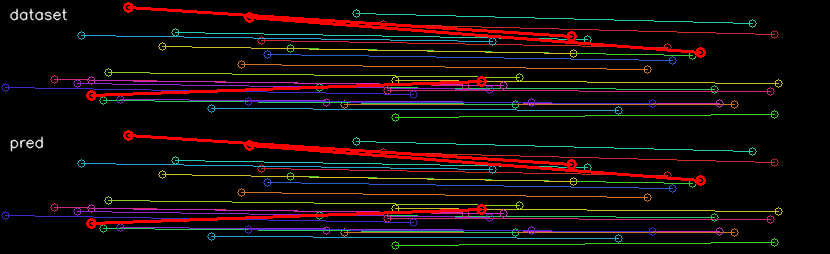
\includegraphics[width=1.0\textwidth]{synthhomo}
	\caption{Outlier detection in homography estimation in synthetic dataset. Top row is ground truth and bottom row is the prediction.}
	\label{fig:synthhomo}
\end{figure}

\begin{figure}[H]
	\centering
	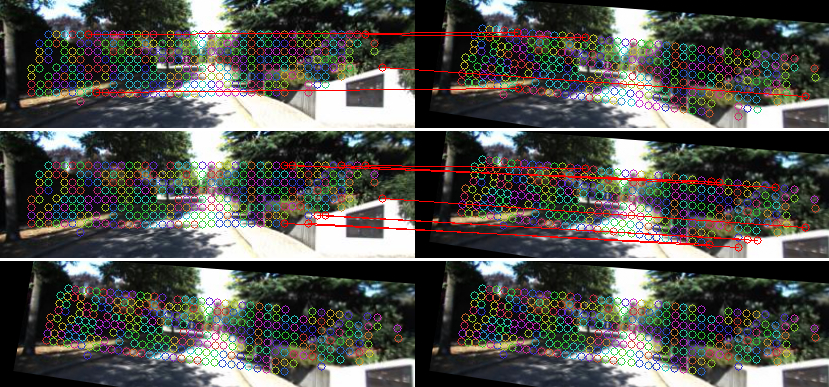
\includegraphics[width=1.0\textwidth]{kittihomo}
	\caption{Outlier detection and homography estimation on images from kitti dataset. First row is from OpenCV findHomography(), second row is from the network, third row is the image from branch A transformed by the homographgy found by OpenCV, fourth row is the image from branch A transformed by the homography found by the network.}
	\label{fig:kittihomo}
\end{figure}

\begin{table}[H]
	\centering
	\begin{tabular}{|l|l|l|l|}
		\hline
		Method & HE $\downarrow$ \\
		\hline
		ConsensusNet & ??? \\
		RANSAC & ??? \\
		\hline
	\end{tabular}
	\caption{Metrics for homography estimation.}
	\label{table:pointsbenchmark}
\end{table}

\begin{table}[H]
\centering
\begin{tabular}{l|l|c|c|c}
	\multicolumn{2}{c}{}&\multicolumn{2}{c}{Predicted}&\\
	\cline{3-4}
	\multicolumn{2}{c|}{}&Inlier&Outlier&\multicolumn{1}{c}{Total}\\
	\cline{2-4}
	\multirow{2}{*}{Actual}& Inlier & $TP$ & $FN$ & $TP+FN$\\
	\cline{2-4}
	& Outlier & $FP$ & $TN$ & $FP+TN$\\
	\cline{2-4}
	\multicolumn{1}{c}{} & \multicolumn{1}{c}{Total} & \multicolumn{1}{c}{$TP+FP$} & \multicolumn{    1}{c}{$FN+TN$} & \multicolumn{1}{c}{$N$}\\
\end{tabular}
	\caption{Confusion matrix for inlier/outlier prediction using ConsensusNet.}
	\label{table:consensusconfusion}
\end{table}


\begin{table}[H]
	\centering
	\begin{tabular}{l|l|c|c|c}
		\multicolumn{2}{c}{}&\multicolumn{2}{c}{Predicted}&\\
		\cline{3-4}
		\multicolumn{2}{c|}{}&Inlier&Outlier&\multicolumn{1}{c}{Total}\\
		\cline{2-4}
		\multirow{2}{*}{Actual}& Inlier & $TP$ & $FN$ & $TP+FN$\\
		\cline{2-4}
		& Outlier & $FP$ & $TN$ & $FP+TN$\\
		\cline{2-4}
		\multicolumn{1}{c}{} & \multicolumn{1}{c}{Total} & \multicolumn{1}{c}{$TP+FP$} & \multicolumn{    1}{c}{$FN+TN$} & \multicolumn{1}{c}{$N$}\\
	\end{tabular}
	\caption{Confusion matrix for inlier/outlier prediction using RANSAC.}
	\label{table:consensusconfusion}
\end{table}

TODO: Insert actual numbers from the testing code and describe what the results are showing....